\documentclass{standalone}
\usepackage{fontspec}
\usepackage[dvipsnames]{xcolor}
\usepackage{tikz}

\tikzset{numnode/.style={draw, ultra thick, minimum size=0.75in, inner sep=0pt}}
\tikzset{circnode/.style={draw, black, line width=1.0mm, circle, minimum size=0.75in, inner sep=0pt, fill=white}}
\tikzset{pcbwire/.style={draw, black, line width=1.5mm}}


\begin{document}
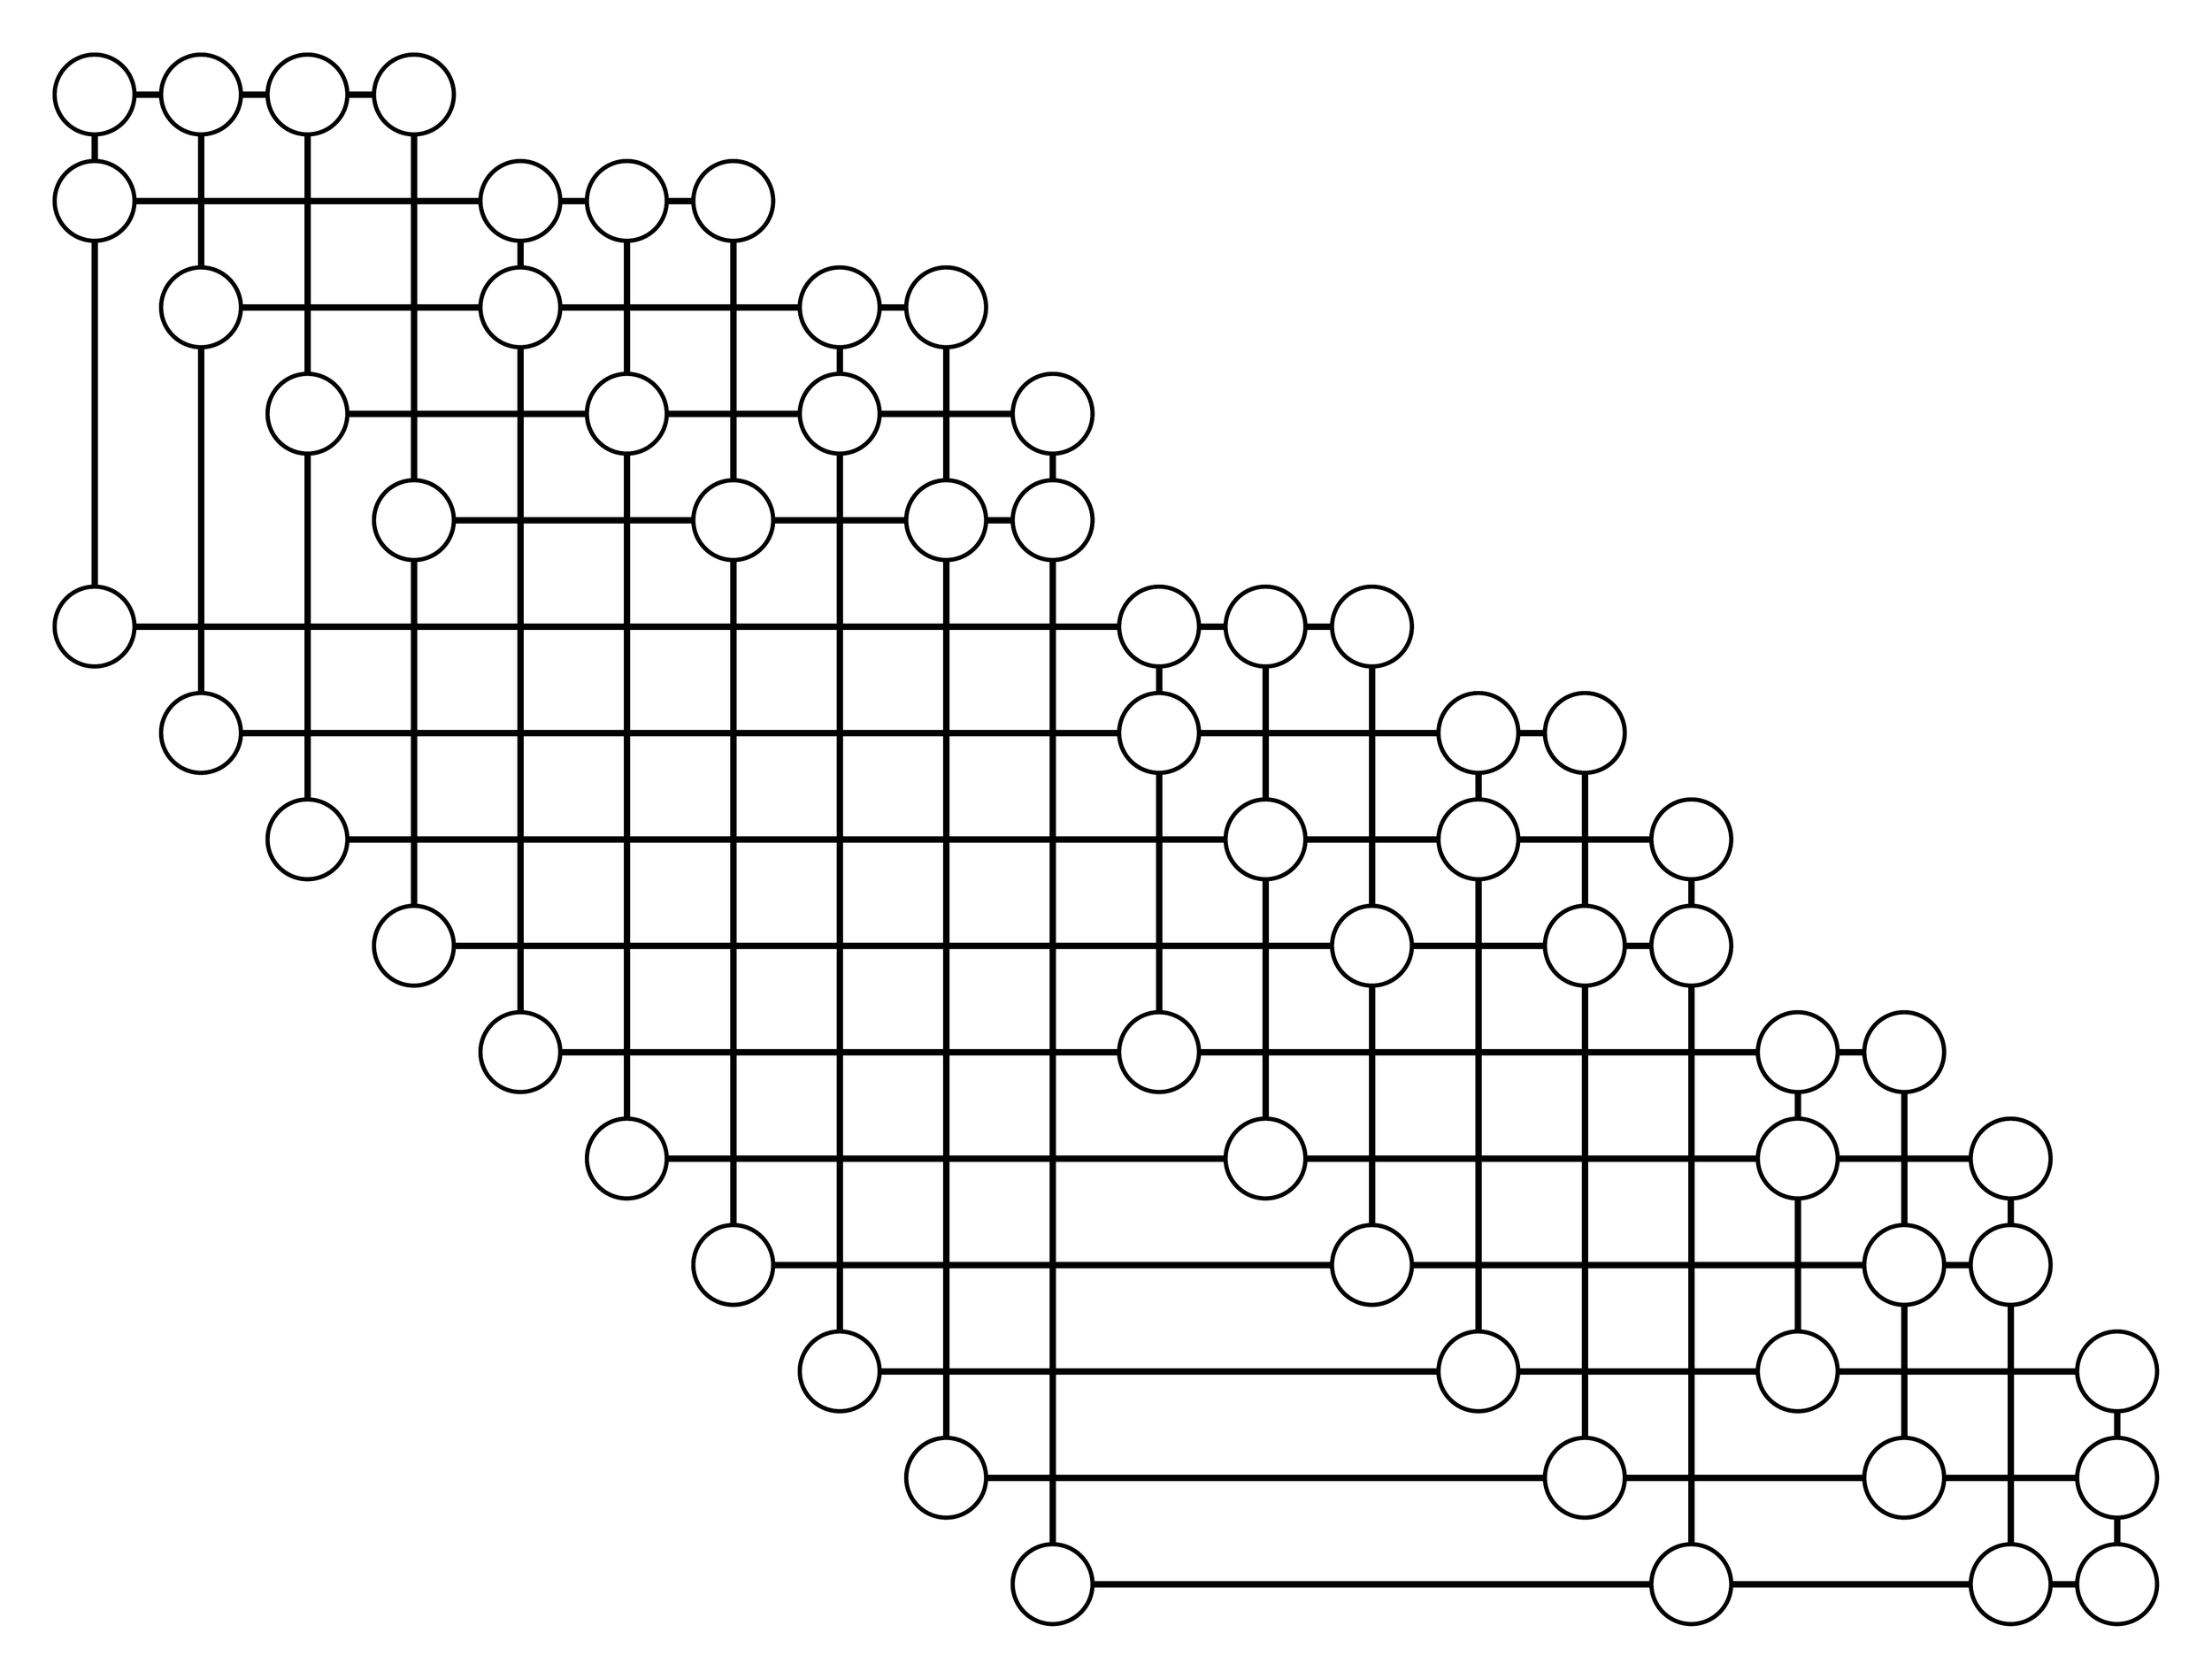
\begin{tikzpicture}[x=1in, y=1in]
\setmainfont[Scale=2.0]{Glass Antiqua}
\Huge
\path[fill=white] (-0.75,0.75) rectangle (19.75, -14.75);

%\foreach \i in {0,-1,...,-14}
%	\draw[line width=1.5mm, black] (0,\i) -- (19,\i);
%
%\foreach \i in {0,1,...,19}
%	\draw[line width=1.5mm, black] (\i,0) -- (\i,-14);
	
%\foreach \i in {-12,-13,...,-14} {
%\node[numnode] at (-5.0,\i) {1};
%\node[numnode] at (-4.25,\i) {2};
%\node[numnode] at (-3.5,\i) {3};
%\node[numnode] at (-2.75,\i) {4};
%\node[numnode] at (-2.0,\i) {5};
%\node[numnode] at (-1.25,\i) {6};
%}

% Row Labels
%\node[numnode] at (-5.0,0) {1};
%\node[numnode] at (-4.25,0) {2};
%
%\node[numnode] at (-5.0,-1) {1};
%\node[numnode] at (-3.5,-1) {3};
%
%\node[numnode] at (-5.0,-2) {1};
%\node[numnode] at (-2.75,-2) {4};
%
%\node[numnode] at (-5.0,-3) {1};
%\node[numnode] at (-2.0,-3) {5};
%
%\node[numnode] at (-5.0,-4) {1};
%\node[numnode] at (-1.25,-4) {6};
%
%\node[numnode] at (-4.25,-5) {2};
%\node[numnode] at (-3.5,-5) {3};
%
%\node[numnode] at (-4.25,-6) {2};
%\node[numnode] at (-2.75,-6) {4};
%
%\node[numnode] at (-4.25,-7) {2};
%\node[numnode] at (-2.0,-7) {5};
%
%\node[numnode] at (-4.25,-8) {2};
%\node[numnode] at (-1.25,-8) {6};
%
%\node[numnode] at (-3.5,-9) {3};
%\node[numnode] at (-2.75,-9) {4};
%
%\node[numnode] at (-3.5,-10) {3};
%\node[numnode] at (-2.0,-10) {5};
%
%\node[numnode] at (-3.5,-11) {3};
%\node[numnode] at (-1.25,-11) {6};
%
%\node[numnode] at (-2.75,-12) {4};
%\node[numnode] at (-2.0,-12) {5};
%
%\node[numnode] at (-2.75,-13) {4};
%\node[numnode] at (-1.25,-13) {6};
%
%\node[numnode] at (-2.0,-14) {5};
%\node[numnode] at (-1.25,-14) {6};
%
%% Edge Markers
\path[pcbwire] (0,0) -- (3,0);
\path[pcbwire] (0,-1) -- (6,-1);
\path[pcbwire] (1,-2) -- (8,-2);
\path[pcbwire] (2,-3) -- (9,-3);
\path[pcbwire] (3,-4) -- (9,-4);
\path[pcbwire] (0,-5) -- (12,-5);
\path[pcbwire] (1,-6) -- (14,-6);
\path[pcbwire] (2,-7) -- (15,-7);
\path[pcbwire] (3,-8) -- (15,-8);
\path[pcbwire] (4,-9) -- (17,-9);
\path[pcbwire] (5,-10) -- (18,-10);
\path[pcbwire] (6,-11) -- (18,-11);
\path[pcbwire] (7,-12) -- (19,-12);
\path[pcbwire] (8,-13) -- (19,-13);
\path[pcbwire] (9,-14) -- (19,-14);


\path[pcbwire] (0,0) -- (0,-5);
\node[circnode] at (0,0) {};
\node[circnode] at (0,-1) {};
\node[circnode] at (0,-5) {};

\path[pcbwire] (1,0) -- (1,-6);
\node[circnode] at (1,0) {};
\node[circnode] at (1,-2) {};
\node[circnode] at (1,-6) {};

\path[pcbwire] (2,0) -- (2,-7);
\node[circnode] at (2,0) {};
\node[circnode] at (2,-3) {};
\node[circnode] at (2,-7) {};

\path[pcbwire] (3,0) -- (3,-8);
\node[circnode] at (3,0) {};
\node[circnode] at (3,-4) {};
\node[circnode] at (3,-8) {};

\path[pcbwire] (4,-1) -- (4,-9);
\node[circnode] at (4,-1) {};
\node[circnode] at (4,-2) {};
\node[circnode] at (4,-9) {};

\path[pcbwire] (5,-1) -- (5,-10);
\node[circnode] at (5,-1) {};
\node[circnode] at (5,-3) {};
\node[circnode] at (5,-10) {};

\path[pcbwire] (6,-1) -- (6,-11);
\node[circnode] at (6,-1) {};
\node[circnode] at (6,-4) {};
\node[circnode] at (6,-11) {};

\path[pcbwire] (7,-2) -- (7,-12);
\node[circnode] at (7,-2) {};
\node[circnode] at (7,-3) {};
\node[circnode] at (7,-12) {};

\path[pcbwire] (8,-2) -- (8,-13);
\node[circnode] at (8,-2) {};
\node[circnode] at (8,-4) {};
\node[circnode] at (8,-13) {};

\path[pcbwire] (9,-3) -- (9,-14);
\node[circnode] at (9,-3) {};
\node[circnode] at (9,-4) {};
\node[circnode] at (9,-14) {};

\path[pcbwire] (10,-5) -- (10,-9);
\node[circnode] at (10,-5) {};
\node[circnode] at (10,-6) {};
\node[circnode] at (10,-9) {};

\path[pcbwire] (11,-5) -- (11,-10);
\node[circnode] at (11,-5) {};
\node[circnode] at (11,-7) {};
\node[circnode] at (11,-10) {};

\path[pcbwire] (12,-5) -- (12,-11);
\node[circnode] at (12,-5) {};
\node[circnode] at (12,-8) {};
\node[circnode] at (12,-11) {};

\path[pcbwire] (13,-6) -- (13,-12);
\node[circnode] at (13,-6) {};
\node[circnode] at (13,-7) {};
\node[circnode] at (13,-12) {};

\path[pcbwire] (14,-6) -- (14,-13);
\node[circnode] at (14,-6) {};
\node[circnode] at (14,-8) {};
\node[circnode] at (14,-13) {};

\path[pcbwire] (15,-7) -- (15,-14);
\node[circnode] at (15,-7) {};
\node[circnode] at (15,-8) {};
\node[circnode] at (15,-14) {};

\path[pcbwire] (16,-9) -- (16,-12);
\node[circnode] at (16,-9) {};
\node[circnode] at (16,-10) {};
\node[circnode] at (16,-12) {};

\path[pcbwire] (17,-9) -- (17,-13);
\node[circnode] at (17,-9) {};
\node[circnode] at (17,-11) {};
\node[circnode] at (17,-13) {};

\path[pcbwire] (18,-10) -- (18,-14);
\node[circnode] at (18,-10) {};
\node[circnode] at (18,-11) {};
\node[circnode] at (18,-14) {};

\path[pcbwire] (19,-12) -- (19,-14);
\node[circnode] at (19,-12) {};
\node[circnode] at (19,-13) {};
\node[circnode] at (19,-14) {};
%

% Shuffled edge markers
%\path[pcbwire] (4,0) -- (14,0);
%\path[pcbwire] (9,-1) -- (19,-1);
%\path[pcbwire] (0,-2) -- (19,-2);
%\path[pcbwire] (0,-3) -- (16,-3);
%\path[pcbwire] (1,-4) -- (10,-4);
%\path[pcbwire] (2,-5) -- (18,-5);
%\path[pcbwire] (2,-6) -- (7,-6);
%\path[pcbwire] (7,-7) -- (18,-7);
%\path[pcbwire] (5,-8) -- (15,-8);
%\path[pcbwire] (2,-9) -- (19,-9);
%\path[pcbwire] (3,-10) -- (18,-10);
%\path[pcbwire] (3,-11) -- (11,-11);
%\path[pcbwire] (0,-12) -- (17,-12);
%\path[pcbwire] (5,-13) -- (17,-13);
%\path[pcbwire] (1,-14) -- (17,-14);
%
%
%\path[pcbwire] (14,0) -- (14,-5);
%\node[circnode] at (14,0) {};
%\node[circnode] at (14,-1) {};
%\node[circnode] at (14,-5) {};
%
%\path[pcbwire] (4,0) -- (4,-6);
%\node[circnode] at (4,0) {};
%\node[circnode] at (4,-2) {};
%\node[circnode] at (4,-6) {};
%
%\path[pcbwire] (13,0) -- (13,-7);
%\node[circnode] at (13,0) {};
%\node[circnode] at (13,-3) {};
%\node[circnode] at (13,-7) {};
%
%\path[pcbwire] (6,0) -- (6,-8);
%\node[circnode] at (6,0) {};
%\node[circnode] at (6,-4) {};
%\node[circnode] at (6,-8) {};
%
%\path[pcbwire] (19,-1) -- (19,-9);
%\node[circnode] at (19,-1) {};
%\node[circnode] at (19,-2) {};
%\node[circnode] at (19,-9) {};
%
%\path[pcbwire] (16,-1) -- (16,-10);
%\node[circnode] at (16,-1) {};
%\node[circnode] at (16,-3) {};
%\node[circnode] at (16,-10) {};
%
%\path[pcbwire] (9,-1) -- (9,-11);
%\node[circnode] at (9,-1) {};
%\node[circnode] at (9,-4) {};
%\node[circnode] at (9,-11) {};
%
%\path[pcbwire] (0,-2) -- (0,-12);
%\node[circnode] at (0,-2) {};
%\node[circnode] at (0,-3) {};
%\node[circnode] at (0,-12) {};
%
%\path[pcbwire] (10,-2) -- (10,-13);
%\node[circnode] at (10,-2) {};
%\node[circnode] at (10,-4) {};
%\node[circnode] at (10,-13) {};
%
%\path[pcbwire] (1,-3) -- (1,-14);
%\node[circnode] at (1,-3) {};
%\node[circnode] at (1,-4) {};
%\node[circnode] at (1,-14) {};
%
%\path[pcbwire] (2,-5) -- (2,-9);
%\node[circnode] at (2,-5) {};
%\node[circnode] at (2,-6) {};
%\node[circnode] at (2,-9) {};
%
%\path[pcbwire] (18,-5) -- (18,-10);
%\node[circnode] at (18,-5) {};
%\node[circnode] at (18,-7) {};
%\node[circnode] at (18,-10) {};
%
%\path[pcbwire] (11,-5) -- (11,-11);
%\node[circnode] at (11,-5) {};
%\node[circnode] at (11,-8) {};
%\node[circnode] at (11,-11) {};
%
%\path[pcbwire] (7,-6) -- (7,-12);
%\node[circnode] at (7,-6) {};
%\node[circnode] at (7,-7) {};
%\node[circnode] at (7,-12) {};
%
%\path[pcbwire] (5,-6) -- (5,-13);
%\node[circnode] at (5,-6) {};
%\node[circnode] at (5,-8) {};
%\node[circnode] at (5,-13) {};
%
%\path[pcbwire] (15,-7) -- (15,-14);
%\node[circnode] at (15,-7) {};
%\node[circnode] at (15,-8) {};
%\node[circnode] at (15,-14) {};
%
%\path[pcbwire] (12,-9) -- (12,-12);
%\node[circnode] at (12,-9) {};
%\node[circnode] at (12,-10) {};
%\node[circnode] at (12,-12) {};
%
%\path[pcbwire] (8,-9) -- (8,-13);
%\node[circnode] at (8,-9) {};
%\node[circnode] at (8,-11) {};
%\node[circnode] at (8,-13) {};
%
%\path[pcbwire] (3,-10) -- (3,-14);
%\node[circnode] at (3,-10) {};
%\node[circnode] at (3,-11) {};
%\node[circnode] at (3,-14) {};
%
%\path[pcbwire] (17,-12) -- (17,-14);
%\node[circnode] at (17,-12) {};
%\node[circnode] at (17,-13) {};
%\node[circnode] at (17,-14) {};
% 
\end{tikzpicture}
\end{document}
